\documentclass[a4paper,12pt]{extarticle}
\usepackage[utf8x]{inputenc}
\usepackage[T1,T2A]{fontenc}
\usepackage[russian]{babel}
\usepackage{hyperref}
\usepackage{indentfirst}
\usepackage{listings}
\usepackage{color}
\usepackage{here}
\usepackage{array}
\usepackage{multirow}
\usepackage{graphicx}

\usepackage{amsmath}

\usepackage{caption}
\renewcommand{\lstlistingname}{Программа} % заголовок листингов кода

\bibliographystyle{ugost2008ls}

\usepackage{listings}
\lstset{ %
extendedchars=\true,
keepspaces=true,
language=C,						% choose the language of the code
basicstyle=\footnotesize,		% the size of the fonts that are used for the code
numbers=left,					% where to put the line-numbers
numberstyle=\footnotesize,		% the size of the fonts that are used for the line-numbers
stepnumber=1,					% the step between two line-numbers. If it is 1 each line will be numbered
numbersep=5pt,					% how far the line-numbers are from the code
backgroundcolor=\color{white},	% choose the background color. You must add \usepackage{color}
showspaces=false				% show spaces adding particular underscores
showstringspaces=false,			% underline spaces within strings
showtabs=false,					% show tabs within strings adding particular underscores
frame=single,           		% adds a frame around the code
tabsize=2,						% sets default tabsize to 2 spaces
captionpos=t,					% sets the caption-position to top
breaklines=true,				% sets automatic line breaking
breakatwhitespace=false,		% sets if automatic breaks should only happen at whitespace
escapeinside={\%*}{*)},			% if you want to add a comment within your code
postbreak=\raisebox{0ex}[0ex][0ex]{\ensuremath{\color{red}\hookrightarrow\space}},
texcl=true,
inputpath=listings,                     % директория с листингами
}

\usepackage[left=2cm,right=2cm,
top=2cm,bottom=2cm,bindingoffset=0cm]{geometry}

%% Нумерация картинок по секциям
\usepackage{chngcntr}
\counterwithin{figure}{section}
\counterwithin{table}{section}

%%Точки нумерации заголовков
\usepackage{titlesec}
\titlelabel{\thetitle.\quad}
\usepackage[dotinlabels]{titletoc}

%% Оформления подписи рисунка
\addto\captionsrussian{\renewcommand{\figurename}{Рисунок}}
\captionsetup[figure]{labelsep = period}

%% Подпись таблицы
\DeclareCaptionFormat{hfillstart}{\hfill#1#2#3\par}
\captionsetup[table]{format=hfillstart,labelsep=newline,justification=centering,skip=-10pt,textfont=bf}

%% Путь к каталогу с рисунками
\graphicspath{{fig/}}

\begin{document}	% начало документа

% Титульная страница
\begin{titlepage}	% начало титульной страницы

	\begin{center}		% выравнивание по центру

		\large Санкт-Петербургский Политехнический Университет Петра Великого\\
		\large Институт компьютерных наук и технологий \\
		\large Кафедра компьютерных систем и программных технологий\\[6cm]
		% название института, затем отступ 6см
		
		\huge Телекоммуникационные технологии\\[0.5cm] % название работы, затем отступ 0,5см
		\large Отчет по лабораторной работе №4\\[0.1cm]
		\large Аналоговая модуляция\\[5cm]

	\end{center}


	\begin{flushright} % выравнивание по правому краю
		\begin{minipage}{0.25\textwidth} % врезка в половину ширины текста
			\begin{flushleft} % выровнять её содержимое по левому краю

				\large\textbf{Работу выполнил:}\\
				\large Соболь В.О.\\
				\large {Группа:} 33501/4\\
				
				\large \textbf{Преподаватель:}\\
				\large Богач Н.В.

			\end{flushleft}
		\end{minipage}
	\end{flushright}
	
	\vfill % заполнить всё доступное ниже пространство

	\begin{center}
	\large Санкт-Петербург\\
	\large \the\year % вывести дату
	\end{center} % закончить выравнивание по центру

\thispagestyle{empty} % не нумеровать страницу
\end{titlepage} % конец титульной страницы

\vfill % заполнить всё доступное ниже пространство

% Содержание
% Содержание
\renewcommand\contentsname{\centerline{Содержание}}
\tableofcontents
\newpage




\section{Цель работы}
Целью данной работы является приобретение навыков генерации и визуализации сигналов, построение спектра сигналов разложеним этих сигналов в ряд Фурье и определение синхропосылки методом взаимной корреляции.

\section{Постановка задачи}
Задачей работы является:
\begin{enumerate}
\item промоделировать сигналы из Главы 3, сс. 150–170 справочного пособия в Matlab
\item получить их спектр с помощью разложения в ряд Фурье
\item с помощью функции корреляции найти позицию синхропосылки
\end{enumerate}

\section{Теоретическая информация}
\subsection{Аналоговый сигнал}
Аналоговый сигнал, с математической точки зрения, представляет собой функцию времени.
Для визуализации сигнал необходимо дискретизировать, то есть подставить в функцию 
вектор дискретных значений времени (временные отсчёты), и получить вектор значений
функции в этих отсчётах.


\subsection{Затухающие сигналы}
Затухание гармонического сигнала получается умножением на убывающую экспоненциальную функцию:
\begin{equation}
	S = exp^{-\alpha t} * s
\end{equation}
где $s$ --- гармонический сигнал

\subsection{Одиночные импульсы}
Для получения прямоугольных импульсов используется функция 
\begin{eqnarray}
y =
\begin{cases}
1, & \text{если } -\frac{width}{2} \leq t < \frac{width}{2}\\
0, & \text{если } t<-\frac{width}{2} , t \geq \frac{width}{2}
\end{cases}
\end{eqnarray}
$t$---вектор временных отсчётов, $width$---ширина (длительность) импульса.
В Matlab эта функция называется rectpuls.

Для создания треугольных импульсов используется функция
\begin{eqnarray}
y =
\begin{cases}
\frac{2t+width}{width(skew+1)}, & -\frac{width}{2}\leq t < \frac{width*skew}{2}\\
\frac{2t-width}{width(skew-1)}, &  \frac{width*skew}{2}\leq t < \frac{width}{2}\\
0, & |t| > \frac{width}{2}
\end{cases}
\end{eqnarray}
$skew$ - коэффициент асимметрии импульса, $t$---вектор временных отсчётов, $width$---ширина импульса.
В Matlab эта функция называется tripuls.


\subsection{Ограниченная полоса частот}
Для формирование сигнала, с ограниченной полосой частот, используется функция вида:
\begin{eqnarray}
y = \frac{\sin(\pi x)}{\pi x}
\end{eqnarray}
Функция спектра такого сигнала имеет прямоугольный вид:
\begin{eqnarray}
	y =
	\begin{cases}
		1, & |\omega| < \pi \\
		0, & |\omega| > \pi
	\end{cases}
\end{eqnarray}


\subsection{Гауссов радиоимпульс}

Функция для получения радиоимпульса имеет вид:
\begin{eqnarray}
y = \exp(-\alpha t^2)\cos(2\pi f t) & \alpha = -\frac{5(2\pi f *bw)^2}{bwr *\log 10}
\end{eqnarray}
где $t$ --- временные отсчёты, $f$ --- несущая частота, $bw$ --- относительная ширина спектра,
$bwr$ --- уровень в децибелах, по которому производится измерение ширины спектра.

Спектр такого сигнала можно получить с помощью преобразования Фурье.


\subsection{Функция Дирихле}

Функция Дирихле описывается формулой:
\begin{eqnarray}
	diric(x) = \frac{\sin(n x/2)}{n \sin(x/2)}
\end{eqnarray}
В этой функции $n$ --- целое положительное число и определяет порядок.

Функцию Дирихле это периодическая sinc функция, которая имеет вид:
\begin{list}{}{}
\item при чётном значении $n$

\begin{equation}
	diric_n(x) = \sum \limits_{k = -\infty}^{\infty} sinc \bigg( n \bigg( \frac{t}{2\pi} - k \bigg) \bigg)
\end{equation}

\item при нечётном значении $n$

\begin{equation}
	diric_n(x) = \sum \limits_{k = -\infty}^{\infty} (-1)^k sinc \bigg( n \bigg( \frac{t}{2\pi} - k \bigg) \bigg)
\end{equation}
\end{list}


\subsection{Математические законы изменения мгновенной частоты}
В данной работе рассматриваются 3 закона:
\begin{list}{}{}

\item линейный  

\begin{eqnarray}
f(t) = f_0 + \beta t & \beta = \frac{f_1-f_0}{t_1}
\end{eqnarray}

\item квадратичный

\begin{eqnarray}
f(t) = f_0 + \beta t^2 & \beta = \frac{f_1-f_0}{t_1^2}
\end{eqnarray}

\item логарифмический

\begin{eqnarray}
f(t) = f_0 + \exp(\beta t) & \beta = \frac{\ln(f_1-f_0)}{t_1}
\end{eqnarray}

\end{list}

Логарифмический закон противоречит своему названию, т.к. зависимость частоты от времени в нем экспоненциальная.


\subsection{Преобразование Фурье}
Для нахождение спектра сигнала чаще всего применяют преобразование Фурье.
Формула прямого преобразования Фурье выглядит следующим образом:
\begin{equation}
	S(\omega) = \int \limits_{-\infty}^{\infty} s(t)e^{-j\omega t} dt
\end{equation}

Обратное преобразование Фурье строится по следующей формуле:
\begin{equation}
	s(t) = \frac{1}{2\pi} \int \limits_{-\infty}^{\infty} S(\omega)e^{j\omega t} d\omega
\end{equation}

\subsection{Взаимная корреляция}
Для нахождения синхропосылки в сигнале используется метод взаимной корреляции. 
Значение корреляции двух векторов $x$ и $y$ строится по формуле:
\begin{equation}
	R = \frac {1}{N} \sum \limits_{i=1}^{N} x_i * y_i
\end{equation}
Если искомая посылка у короче передаваемого вектора х, то она дополняется нулями до необходимой длины.

Если вектор $x$ это сигнал, вектор $y$ --- искомая посылка, а $N$ --- длина сигнала, то для поиска позиции посылки 
в сигнале $N$ раз повторяется вычисление корреляции между $x$ и $y$ и сдвиг $y$.
Максимальные значения в полученном векторе корреляций соответствуют сдвигу, при котором была найдена часть
сигнала $x$ максимально похожая на искомую посылку.

Для ускорения вычисления корреляции, особенно для больших посылках, применяется метод быстрой корреляции:
\begin{equation}
	R = \frac{1}{N} F_D^-1 [X^* * Y]
\end{equation}
где $X^*$ - комплексно-сопряженный вектор от вектора преобразования Фурье от посылки х,
 Y - результат преобразования Фурье от вектора искомой посылки, $ F_D^-1$ - обратное преобразование Фурье.

Данная формула позволяет найти вектор значений взаимной корреляции двух векторов быстрее, чем обычный алгоритм.

\section{Ход работы}

\subsection{Генерация затухающего гармонического сигнала}

Затухающий гармонический сигнал и его спектр получены с помощью кода из листинга~\ref{code:module1}.

На графике~\ref{pic:graph1} показаны различные формы представления затухающего гармонического сигнала, построенного
по дискретным отсчетам. На первом графике обычный вид, на втором --- точечное представление, на третьем точки представлены
как отклонения от нуля и на четвёртом --- ступенчатый график.

Спектр представленного выше сигнала (рис.~\ref{pic:spec1}) получен с помощью разложения в ряд Фурье.


\begin{figure}[H]
	\begin{center}
		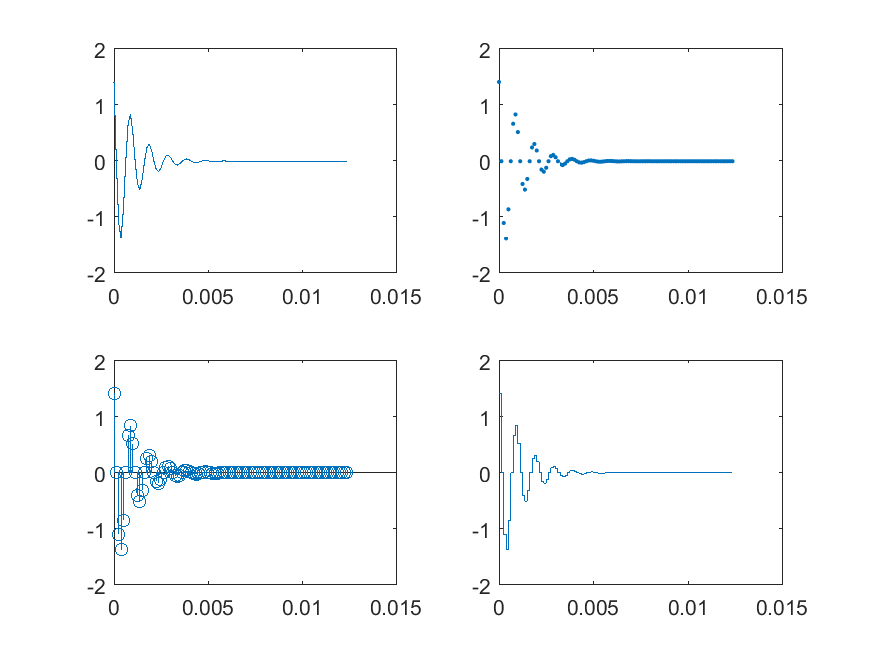
\includegraphics[scale=0.7]{graph1}
		\caption{Графики сигнала} 
		\label{pic:graph1} % название для ссылок внутри кода
	\end{center}
\end{figure}

\begin{figure}[H]
	\begin{center}
		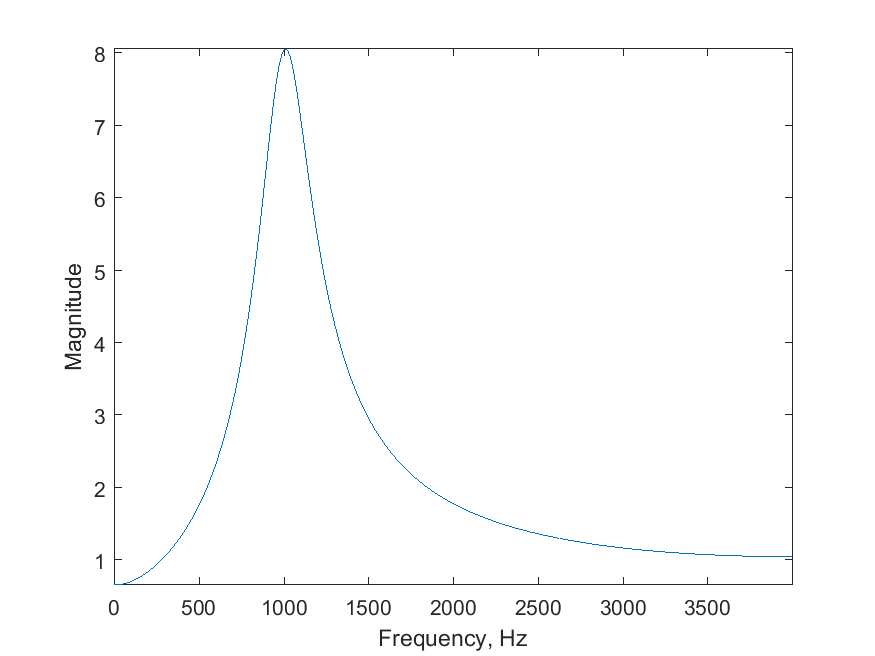
\includegraphics[scale=0.7]{spec1}
		\caption{Спектр сигнала} 
		\label{pic:spec1} % название для ссылок внутри кода
	\end{center}
\end{figure}

\subsection{Многоканальный сигнал}

Несколько сигналов, различающихся по частоте (рис.~\ref{pic:graph2}) получены с помощью кода из листинга~\ref{code:module2}. 
Их спектр приведен на рис.\ref{pic:spec2}.

\begin{figure}[H]
	\begin{center}
		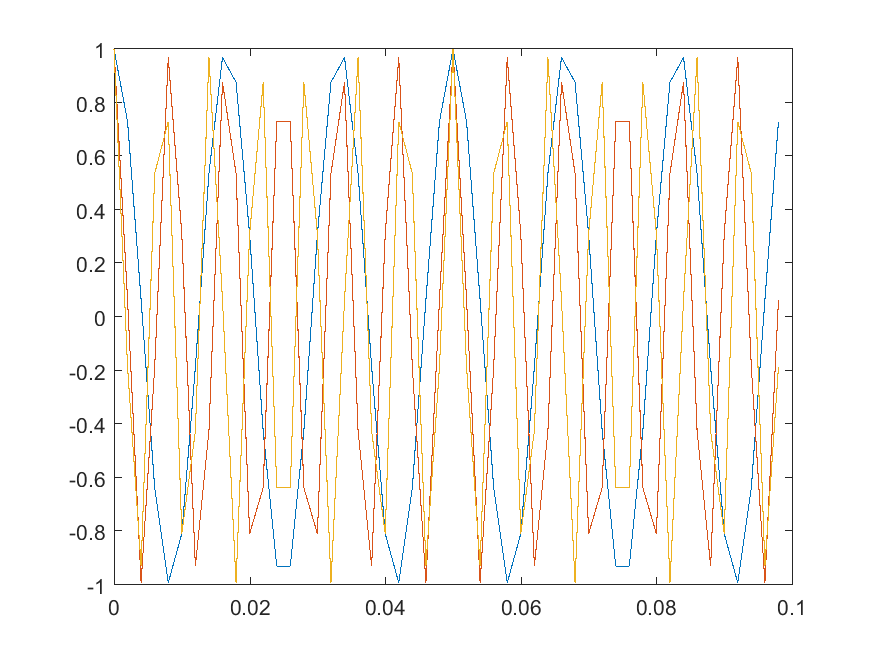
\includegraphics[scale=0.7]{graph2}
		\caption{График сигналов} 
		\label{pic:graph2} % название для ссылок внутри кода
	\end{center}
\end{figure}

\begin{figure}[H]
	\begin{center}
		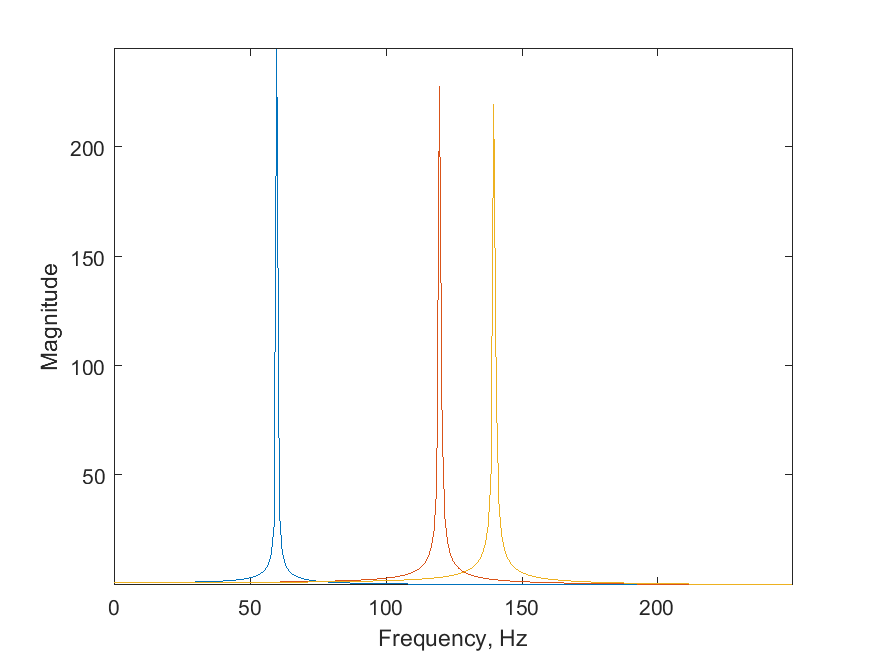
\includegraphics[scale=0.7]{spec2}
		\caption{Спектр сигналов} 
		\label{pic:spec2} % название для ссылок внутри кода
	\end{center}
\end{figure}
\subsection{Кусочные зависимости}

Односторонний экспоненциальный импульс (рис. ~\ref{pic:graph3_1}), прямоугольный импульс (рис. ~\ref{pic:graph3_2}) и несимметричный треугольный импульс (рис. ~\ref{pic:graph3_3}) получены с помощью кода из листинга~\ref{code:module3} согласно заданным уравнениям. Спектры сигналов представлены на рисунках \ref{pic:graph3_1} — \ref{pic:graph3_3}.

\begin{figure}[H]
	\begin{center}
		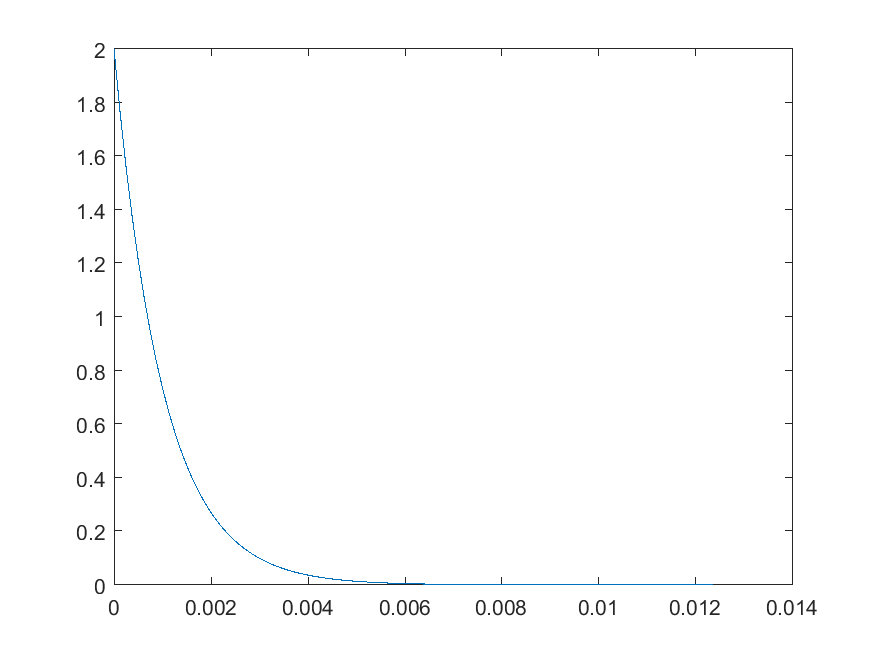
\includegraphics[scale=0.7]{graph3_1}
		\caption{Экспоненциальный импульс} 
		\label{pic:graph3_1} % название для ссылок внутри кода
	\end{center}
\end{figure}
\begin{figure}[H]
	\begin{center}
		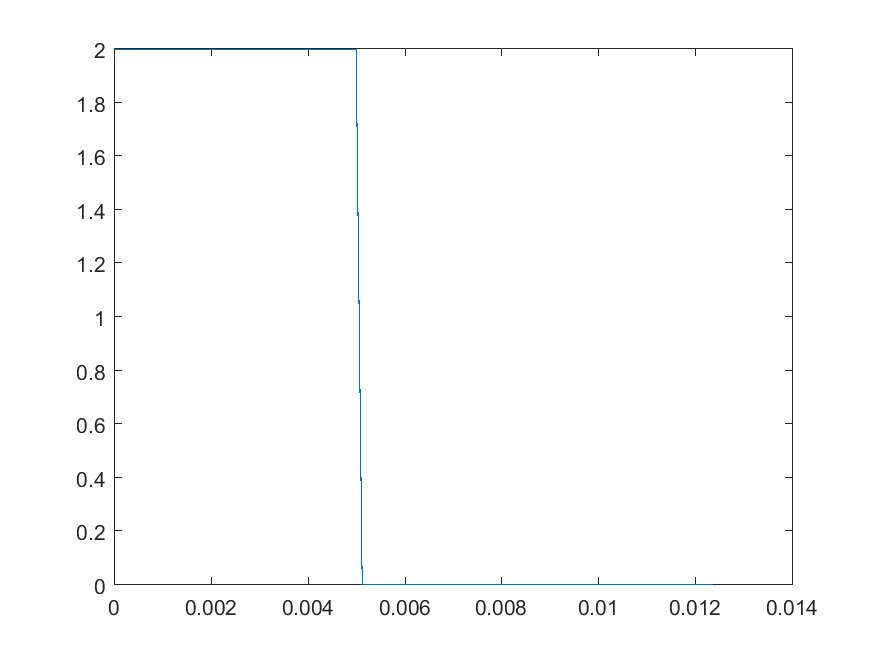
\includegraphics[scale=0.7]{graph3_2}
		\caption{Прямоугольный импульс} 
		\label{pic:graph3_2} % название для ссылок внутри кода
	\end{center}
\end{figure}
\begin{figure}[H]
	\begin{center}
		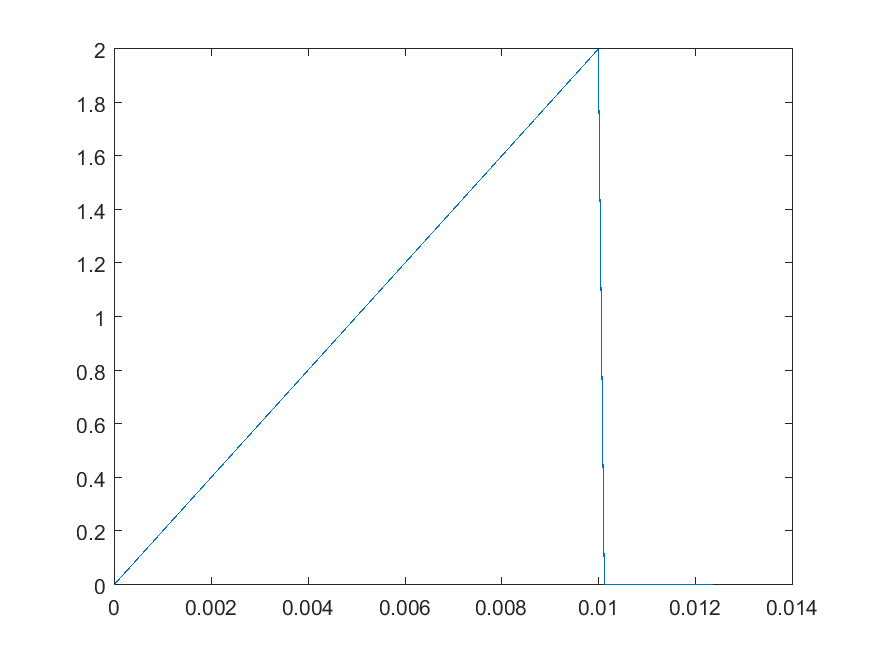
\includegraphics[scale=0.7]{graph3_3}
		\caption{Несимметричный треугольный импульс} 
		\label{pic:graph3_3} % название для ссылок внутри кода
	\end{center}
\end{figure}

\begin{figure}[H]
	\begin{center}
		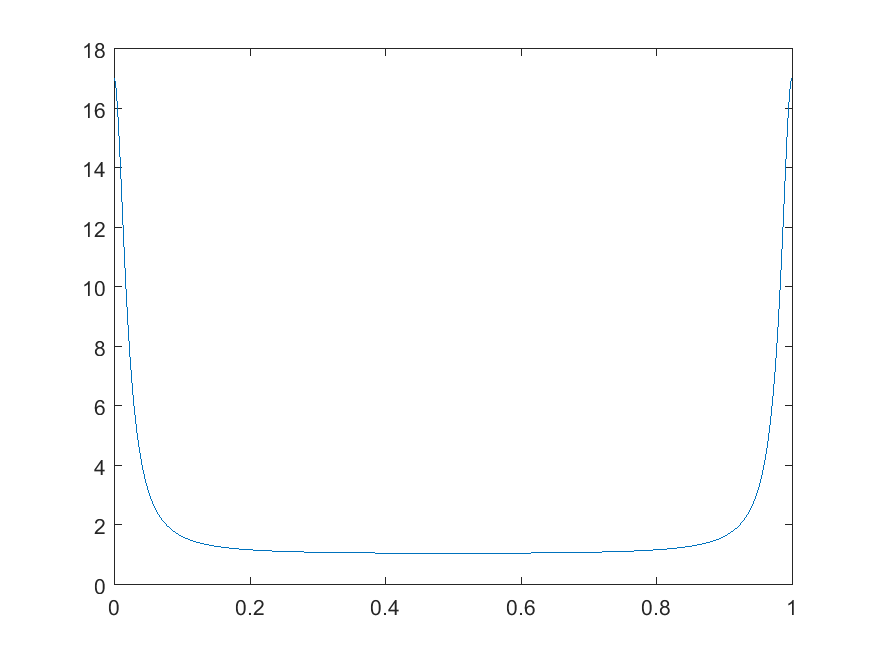
\includegraphics[scale=0.7]{spec3_1}
		\caption{Спектр экспоненциального импульса} 
		\label{pic:spec3_1} % название для ссылок внутри кода
	\end{center}
\end{figure}
\begin{figure}[H]
	\begin{center}
		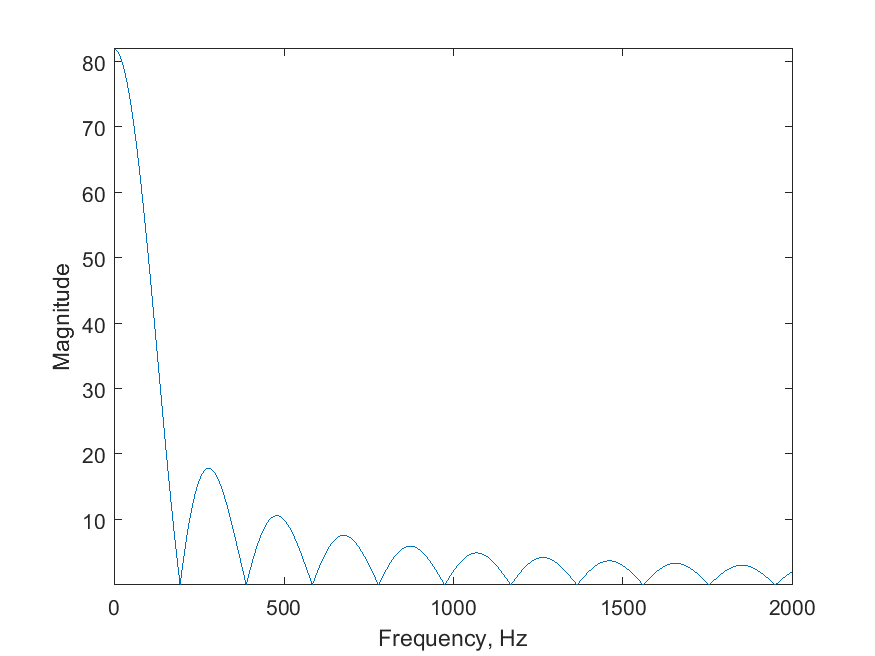
\includegraphics[scale=0.7]{spec3_2}
		\caption{Спектр прямоугольного импульса} 
		\label{pic:spec3_2} % название для ссылок внутри кода
	\end{center}
\end{figure}
\begin{figure}[H]
	\begin{center}
		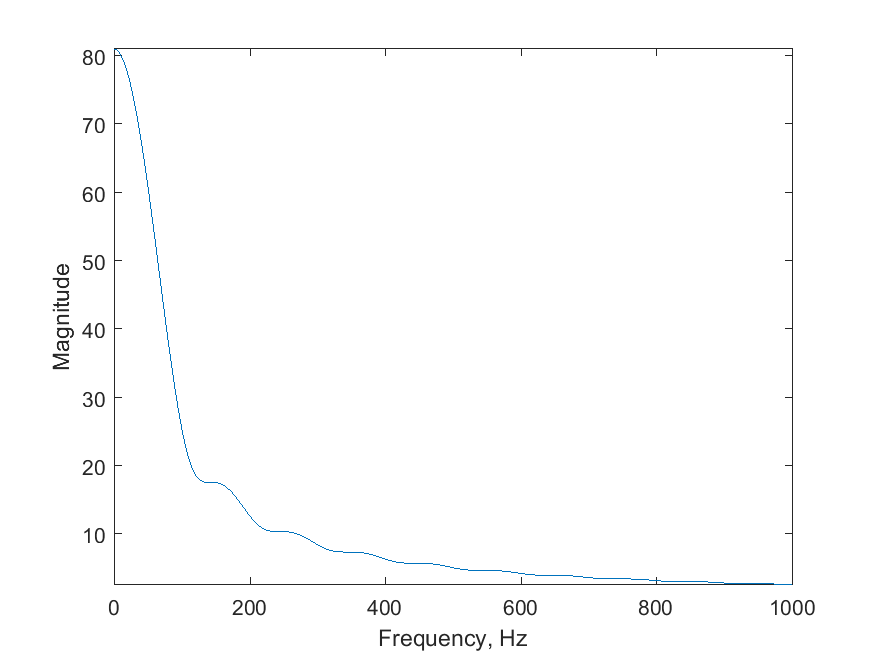
\includegraphics[scale=0.7]{spec3_3}
		\caption{Спектр несимметричного треугольного импульса} 
		\label{pic:spec3_3} % название для ссылок внутри кода
	\end{center}
\end{figure}

\subsection{Прямоугольный импульс}

Сигнал (рис.~\ref{pic:graph4}) генерируется путем соединения двух прямоугольных импульсов, с использованием встроенной функции rectpuls (листинг~\ref{code:module5}). Спектр (рис.~\ref{pic:spec4}) прямоугольного импульса получен разложением сигнала в ряд Фурье.

\begin{figure}[H]
	\begin{center}
		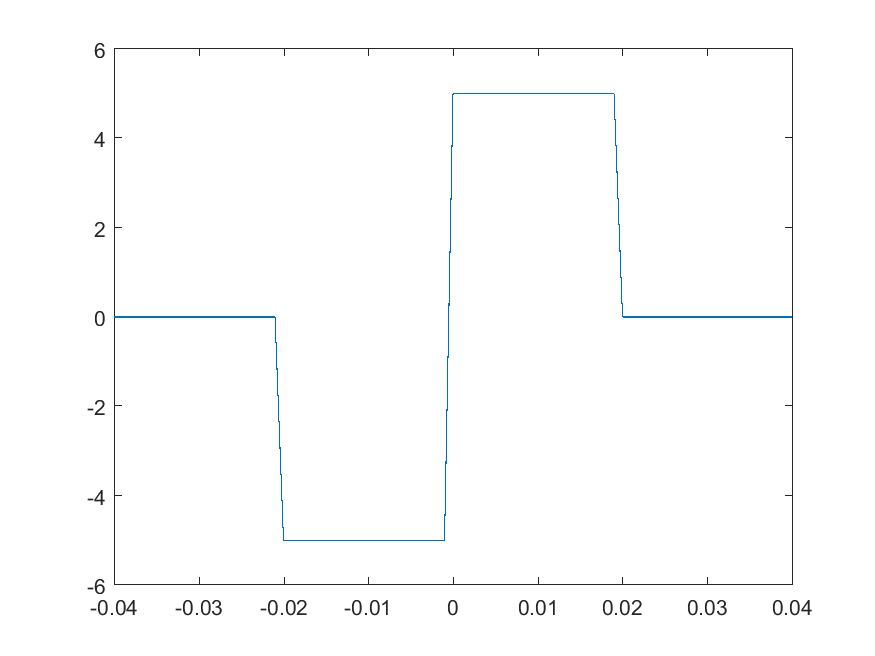
\includegraphics[scale=0.7]{graph4}
		\caption{Прямоугольные импульсы} 
		\label{pic:graph4} % название для ссылок внутри кода
	\end{center}
\end{figure}

\begin{figure}[H]
	\begin{center}
		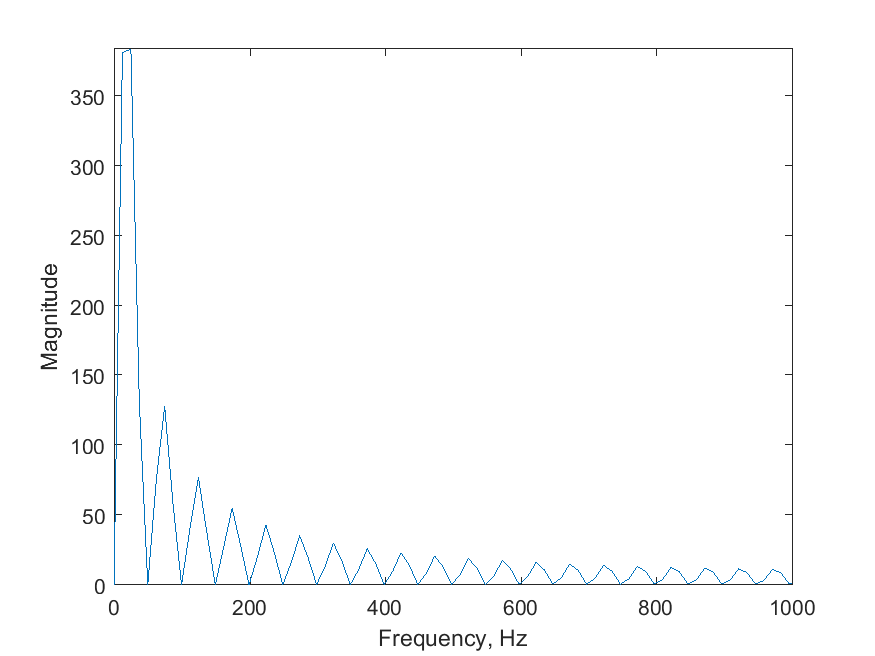
\includegraphics[scale=0.7]{spec4}
		\caption{Спектр прямоугольных импульсов} 
		\label{pic:spec4} % название для ссылок внутри кода
	\end{center}
\end{figure}

\subsection{Трапециевидный импульс}

Трапециевидный сигнал (рис.~\ref{pic:graph5}) генерируется разностью двух треугольных импульсов,
 с использованием встроенной функции tripuls (листинг~\ref{code:module6}).

\begin{figure}[H]
	\begin{center}
		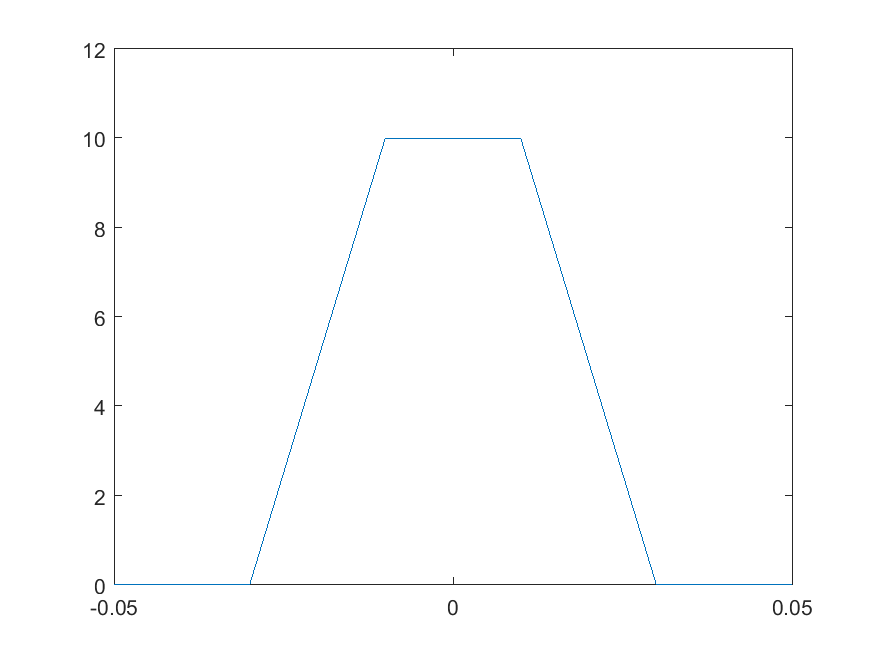
\includegraphics[scale=0.7]{graph5}
		\caption{Трапециевидный импульс} 
		\label{pic:graph5} % название для ссылок внутри кода
	\end{center}
\end{figure}

\begin{figure}[H]
	\begin{center}
		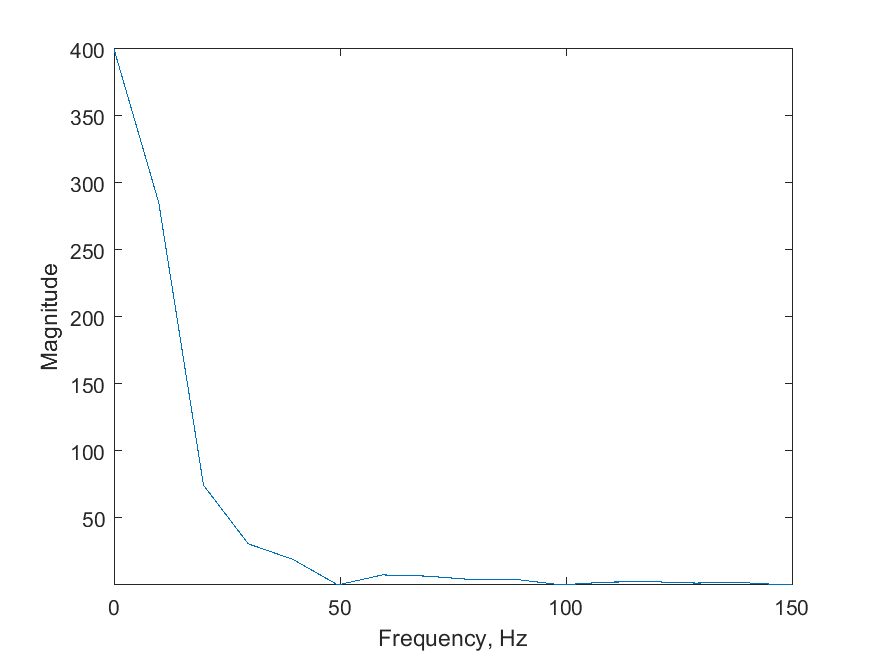
\includegraphics[scale=0.7]{spec5}
		\caption{Спектр трапециевидного импульса} 
		\label{pic:spec5} % название для ссылок внутри кода
	\end{center}
\end{figure}

\subsection{Импульс с ограниченной полосой частот}

Сигнал, у которого спектр ограничен по частоте (рис.~\ref{pic:graph6_1}), получен с помощью программы из листинга~\ref{code:module7}. 
Спектр сигнала (рис.~\ref{pic:graph6_2}) получен с помощь функции sinc.

\begin{figure}[H]
	\begin{center}
		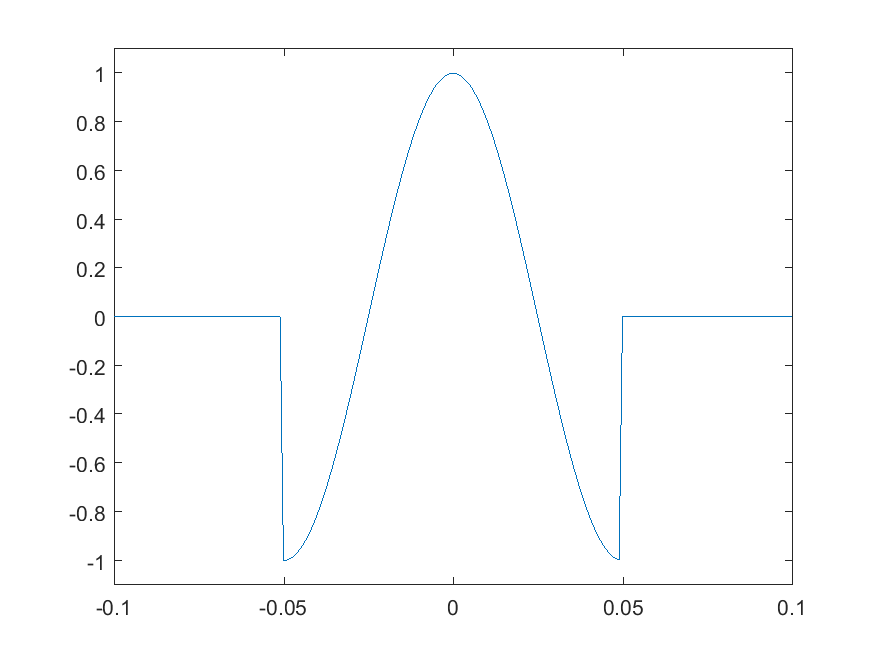
\includegraphics[scale=0.7]{graph6_1}
		\caption{Сигнал с ограниченным спектром} 
		\label{pic:graph6_1} % название для ссылок внутри кода
	\end{center}
\end{figure}
\begin{figure}[H]
	\begin{center}
		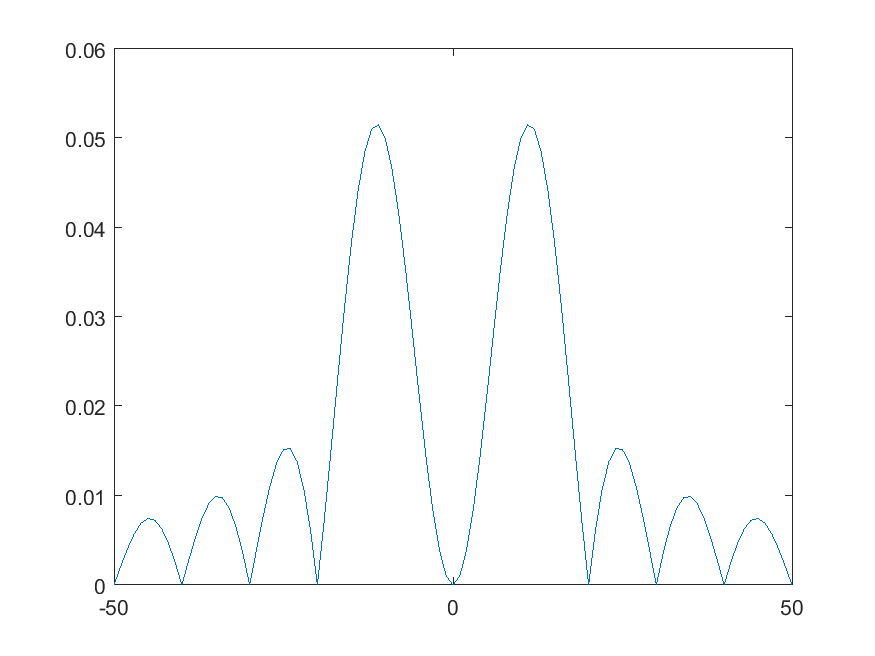
\includegraphics[scale=0.7]{graph6_2}
		\caption{Спектр сигнала с ограниченным спектром} 
		\label{pic:graph6_2} % название для ссылок внутри кода
	\end{center}
\end{figure}

\subsection{Гауссов радиоимпульс}

Гауссов радиоимпульс получен с помощью встроенной функции gauspuls (~\ref{code:module8}). 
\begin{figure}[H]
	\begin{center}
		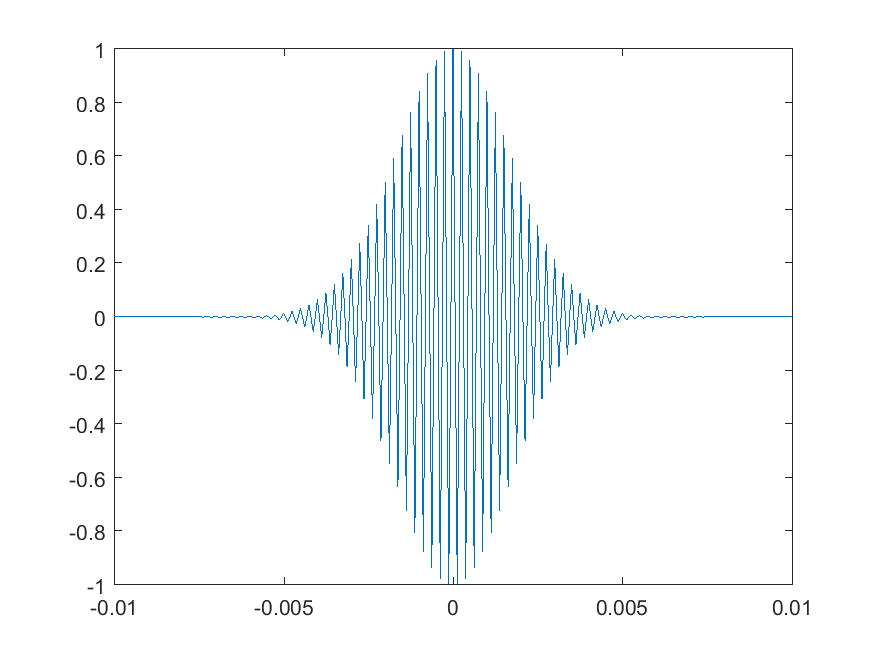
\includegraphics[scale=0.7]{graph7_1}
		\caption{Гауссов радиоимпульс} 
		\label{pic:graph7_1} % название для ссылок внутри кода
	\end{center}
\end{figure}
\begin{figure}[H]
	\begin{center}
		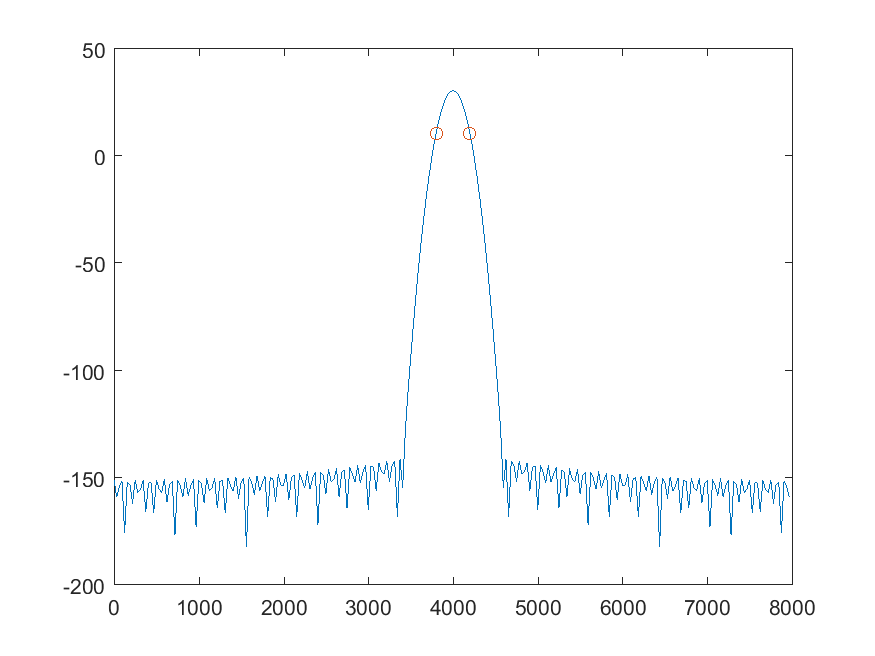
\includegraphics[scale=0.7]{graph7_2}
		\caption{Амплитудный спектр радиоимпульса} 
		\label{pic:graph7_2} % название для ссылок внутри кода
	\end{center}
\end{figure}
На графике спектра (рис.~\ref{pic:graph7_2}) также отмечены расчетные границы этого спектра.

\subsection{Последовательности импульсов}

Треугольные импульсы (рис.~\ref{pic:graph8_1}), получены функцией pulstran (листинг~\ref{code:module9}), которая 
генерирует треугольные импульсы с заданными амплитудами и через заданные промежутки времени. Спектр этого сигнала 
показан на рис.~\ref{pic:spec8_1}.

\begin{figure}[H]
	\begin{center}
		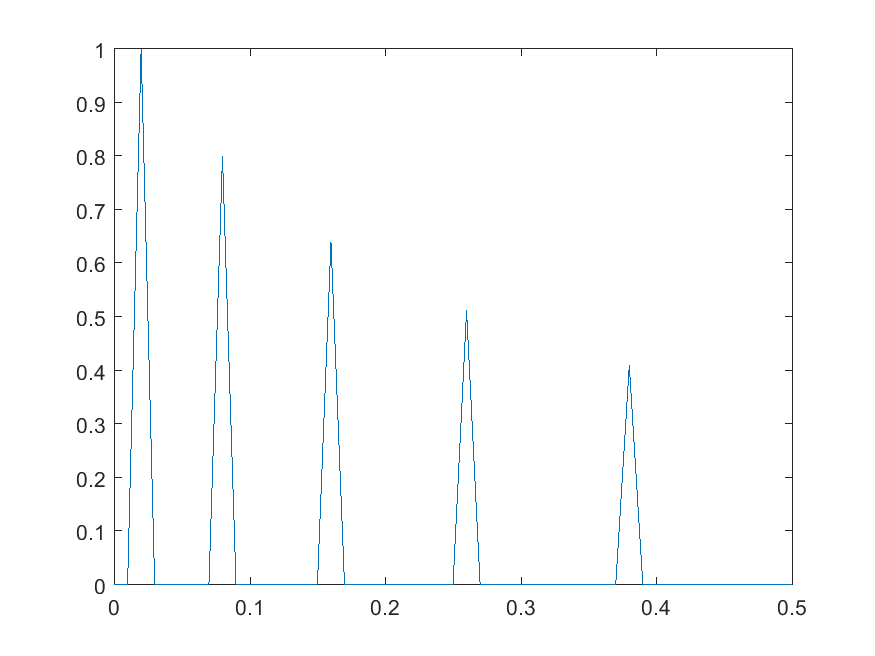
\includegraphics[scale=0.7]{graph8_1}
		\caption{Треугольные импульсы} 
		\label{pic:graph8_1} % название для ссылок внутри кода
	\end{center}
\end{figure}
\begin{figure}[H]
	\begin{center}
		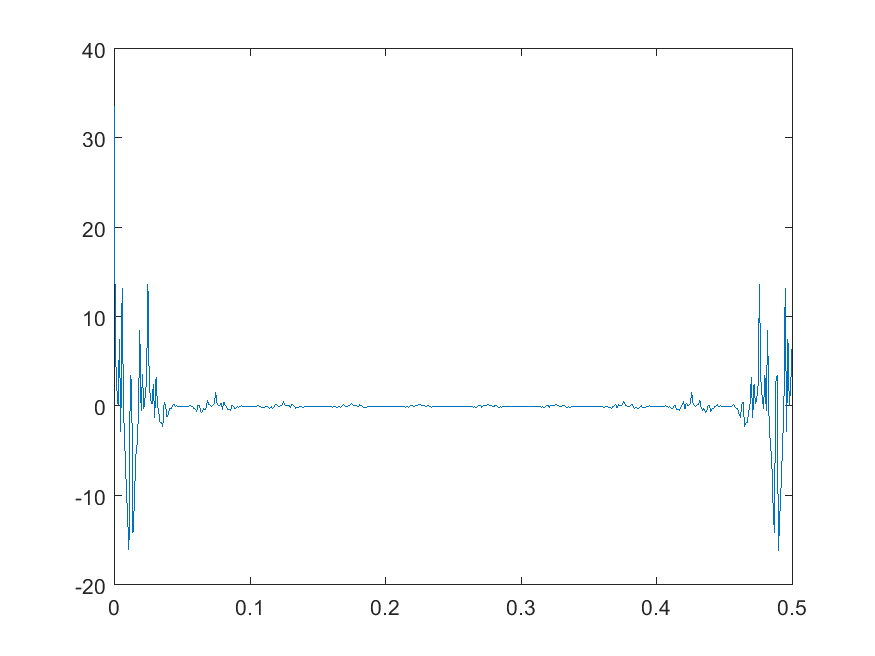
\includegraphics[scale=0.7]{spec8_1}
		\caption{Спектр треугольных импульсов} 
		\label{pic:spec8_1} % название для ссылок внутри кода
	\end{center}
\end{figure}

Гармонические импульсы получены функцией pulstran (листинг~\ref{code:module10}) из вектора отсчетов одиночного импульса.
\begin{figure}[H]
	\begin{center}
		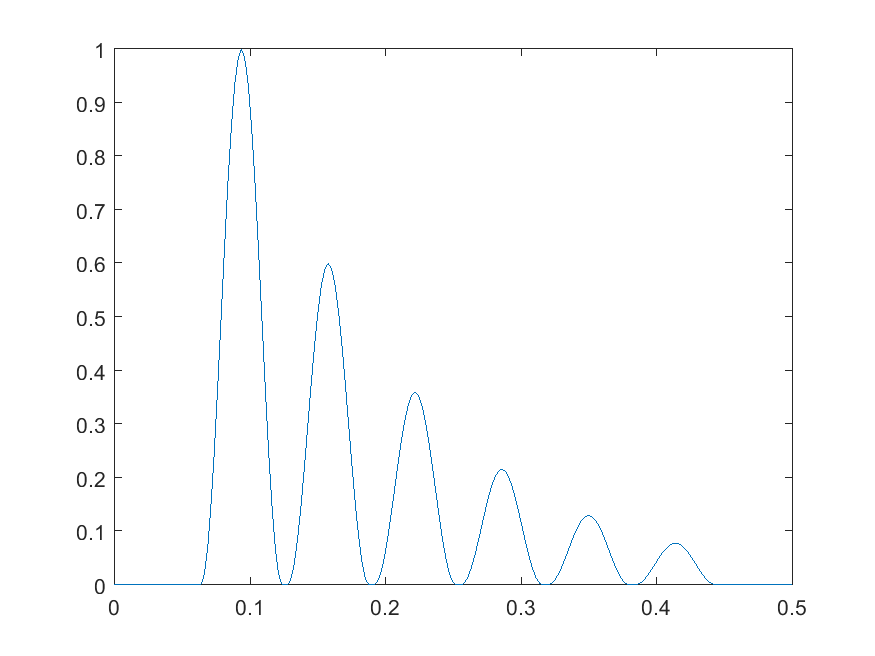
\includegraphics[scale=0.7]{graph8_2}
		\caption{Гармонические импульсы} 
		\label{pic:graph8_2} % название для ссылок внутри кода
	\end{center}
\end{figure}

\begin{figure}[H]
	\begin{center}
		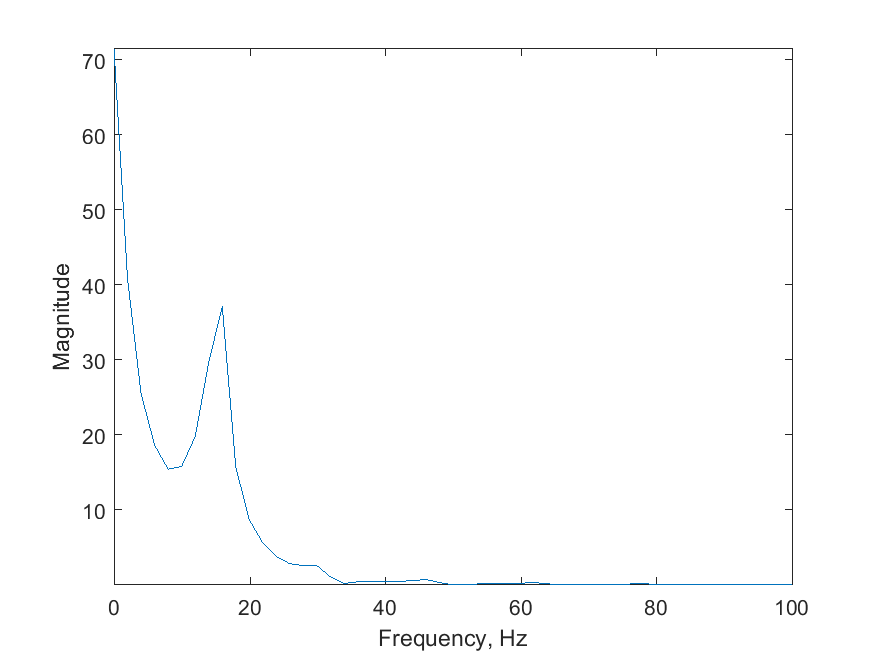
\includegraphics[scale=0.7]{spec8_2}
		\caption{Спектр гармонических импульсов} 
		\label{pic:spec8_2} % название для ссылок внутри кода
	\end{center}
\end{figure}

\subsection{Генерация периодических сигналов}

Периодически повторяющиеся прямоугольные сигналы, созданы с помощью функции square (листинг~\ref{code:module11}).

\begin{figure}[H]
	\begin{center}
		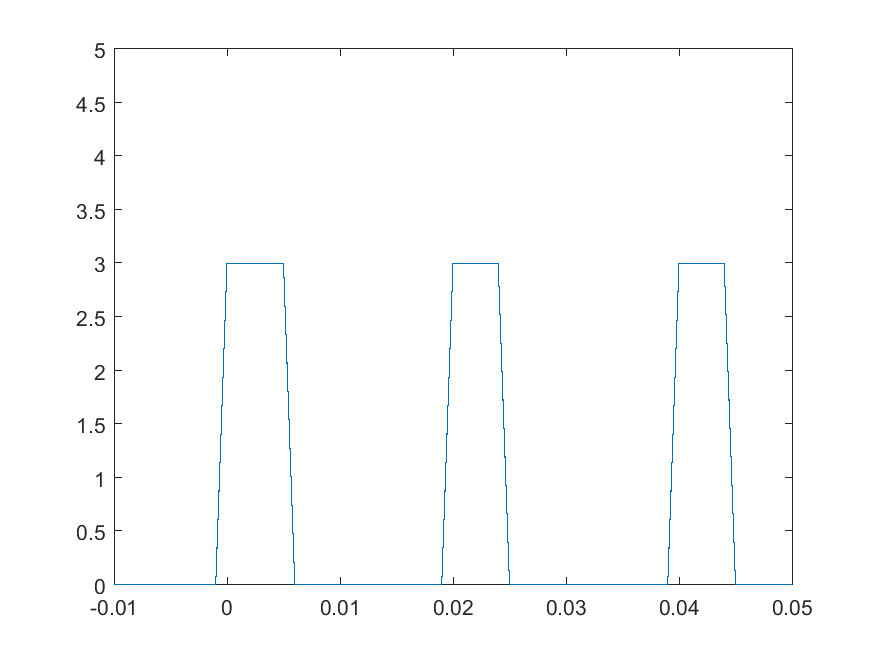
\includegraphics[scale=0.7]{graph9_1}
		\caption{Периодические прямоугольные импульсы} 
		\label{pic:graph9_1} % название для ссылок внутри кода
	\end{center}
\end{figure}

Импульсы обладают одинаковой длительностью и временем паузы между ними.

\begin{figure}[H]
	\begin{center}
		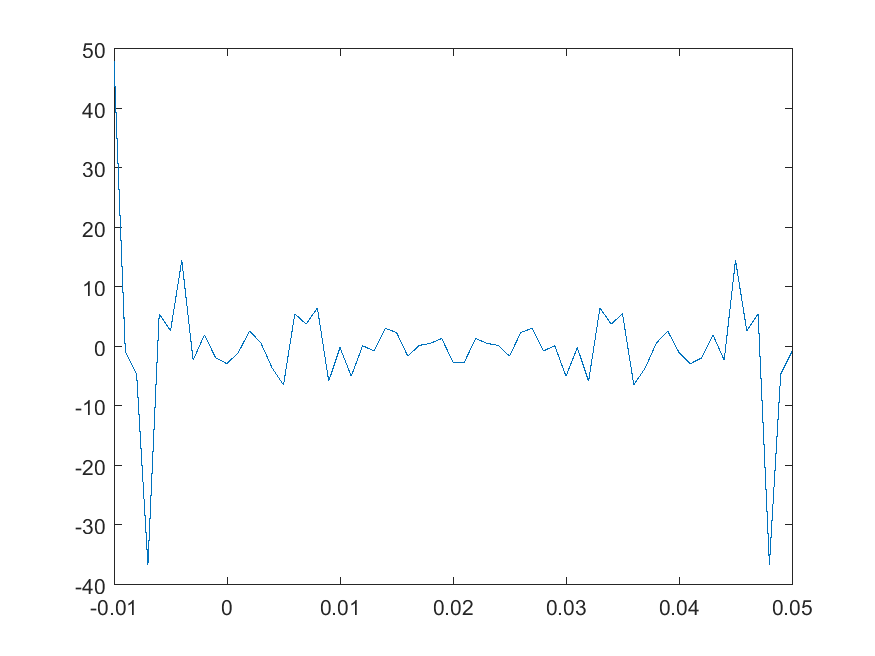
\includegraphics[scale=0.7]{spec9_1}
		\caption{Спектр прямоугольных импульсов} 
		\label{pic:spec9_1} % название для ссылок внутри кода
	\end{center}
\end{figure}

Импульсы треугольной формы с заданными параметрами получены с помощью функции sawtooth (листинг~\ref{code:module12}).

\begin{figure}[H]
	\begin{center}
		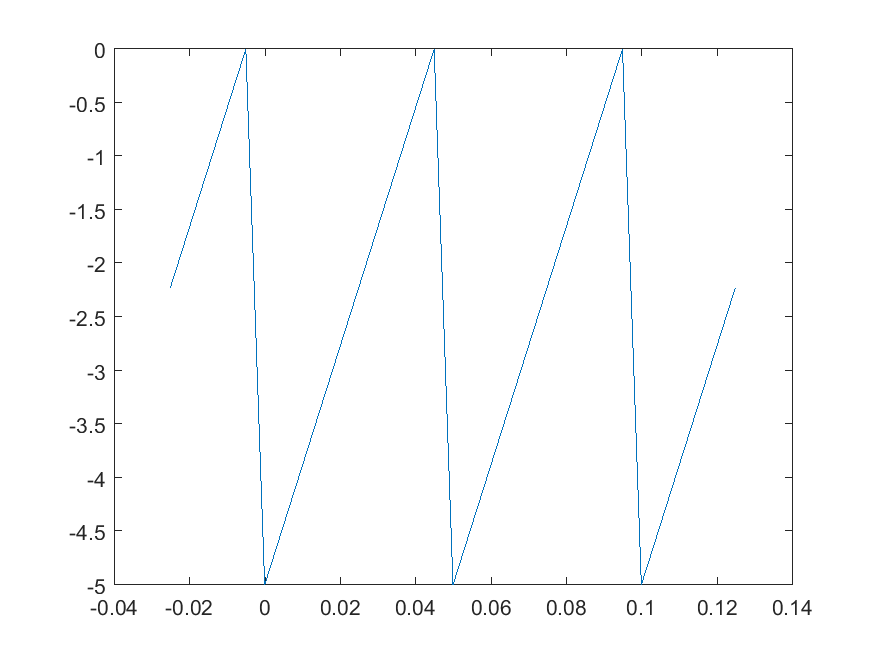
\includegraphics[scale=0.7]{graph9_2}
		\caption{Треугольные импульсы} 
		\label{pic:graph9_2} % название для ссылок внутри кода
	\end{center}
\end{figure}
\begin{figure}[H]
	\begin{center}
		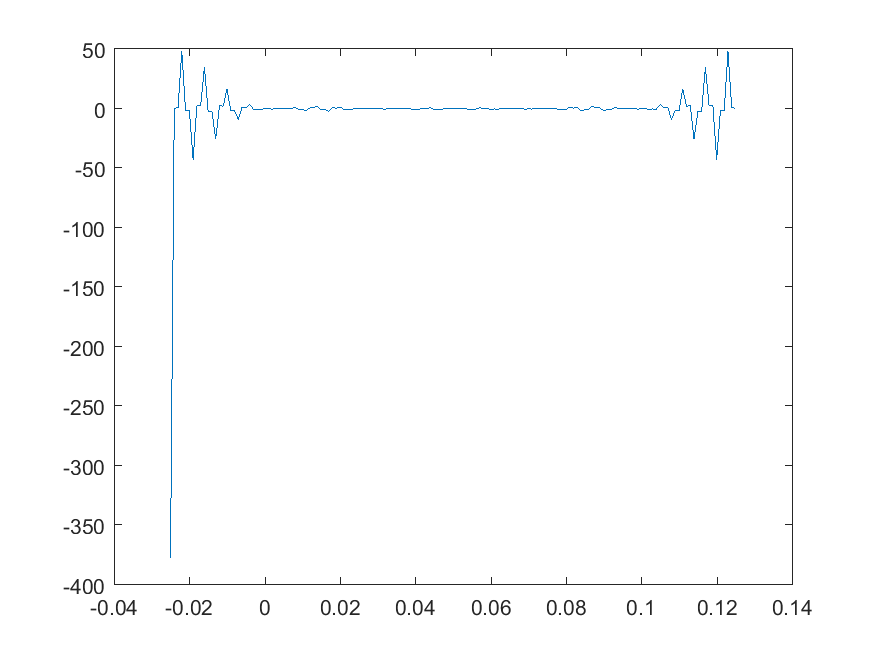
\includegraphics[scale=0.7]{spec9_2}
		\caption{Спектр треугольных импульсов} 
		\label{pic:spec9_2} % название для ссылок внутри кода
	\end{center}
\end{figure}

\subsection{Функция Дирихле}

Для создания выборки из функции Дирихле с четным и нечетным значением параметра использована 
функция diric (листинг~\ref{code:module13}).

\begin{figure}[H]
	\begin{center}
		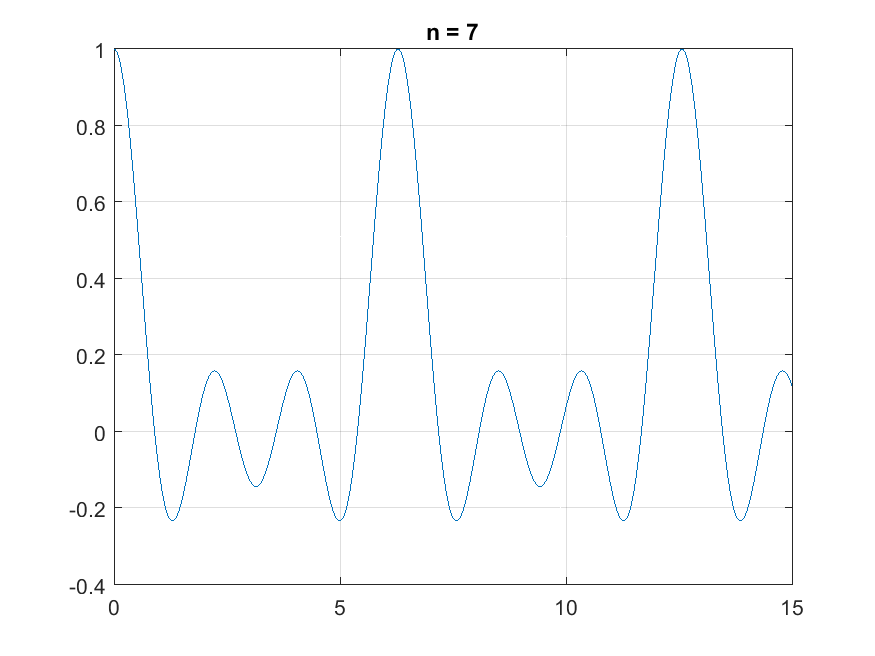
\includegraphics[scale=0.7]{graph10_1}
		\caption{Функция Дирихле с параметром равным 7} 
		\label{pic:graph10_1} % название для ссылок внутри кода
	\end{center}
\end{figure}
\begin{figure}[H]
	\begin{center}
		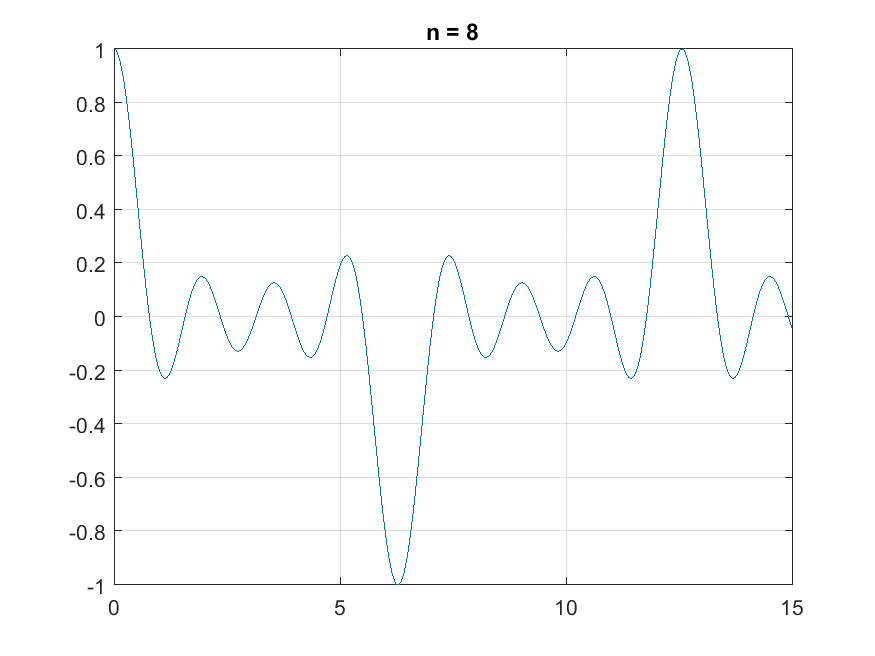
\includegraphics[scale=0.7]{graph10_2}
		\caption{Функция Дирихле с параметром равным 8} 
		\label{pic:graph10_2} % название для ссылок внутри кода
	\end{center}
\end{figure}
Видно, что нечетный параметр обеспечивает однонаправленные импульсы, а частота колебаний растёт с увеличением значения параметра.

\begin{figure}[H]
	\begin{center}
		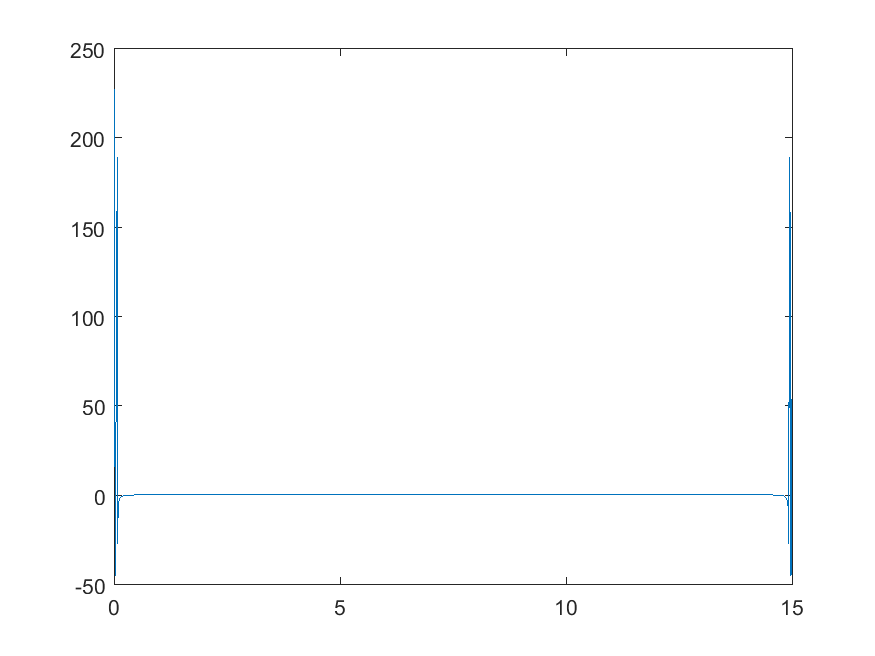
\includegraphics[scale=0.7]{spec10_1}
		\caption{Спектр функции Дирихле с параметром равным 7} 
		\label{pic:spec10_1} % название для ссылок внутри кода
	\end{center}
\end{figure}
\begin{figure}[H]
	\begin{center}
		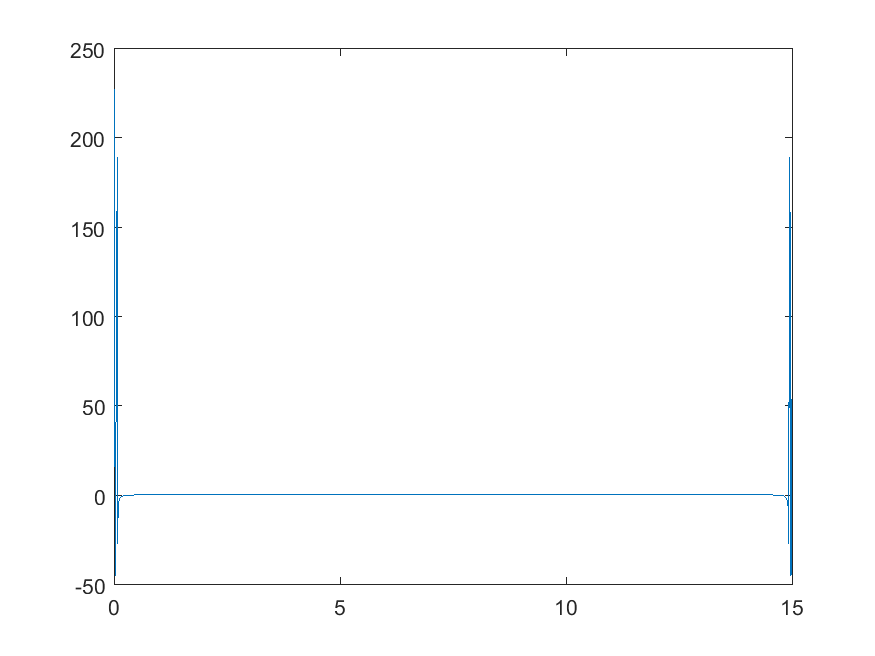
\includegraphics[scale=0.7]{spec10_2}
		\caption{Спектр функции Дирихле с параметром равным 8} 
		\label{pic:spec10_2} % название для ссылок внутри кода
	\end{center}
\end{figure}

\subsection{Сигнал с меняющейся частотой}

Программа, написанная для исследования (листинг~\ref{code:module14}), с помощью функции chirp генерирует колебания, мгновенная частота которых изменяется согласно выбранной функции. В данном примере рассмотрены 3 таких функции — линейная, квадратичная и логарифмическая. На рисунках \ref{pic:graph11_2}, \ref{pic:graph11_2} и \ref{pic:graph11_3} показаны спектрограммы этих сигналов — зависимость мгновенного амплитудного спектра от времени.

\begin{figure}[H]
	\begin{center}
		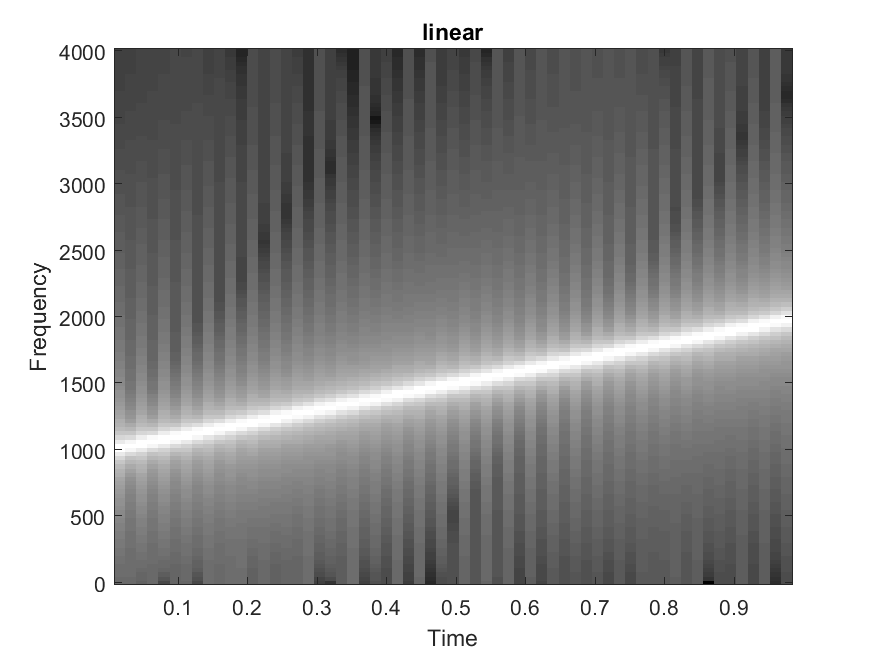
\includegraphics[scale=0.7]{graph11_1}
		\caption{Спектрограмма линейной функции chirp} 
		\label{pic:graph11_1} % название для ссылок внутри кода
	\end{center}
\end{figure}
\begin{figure}[H]
	\begin{center}
		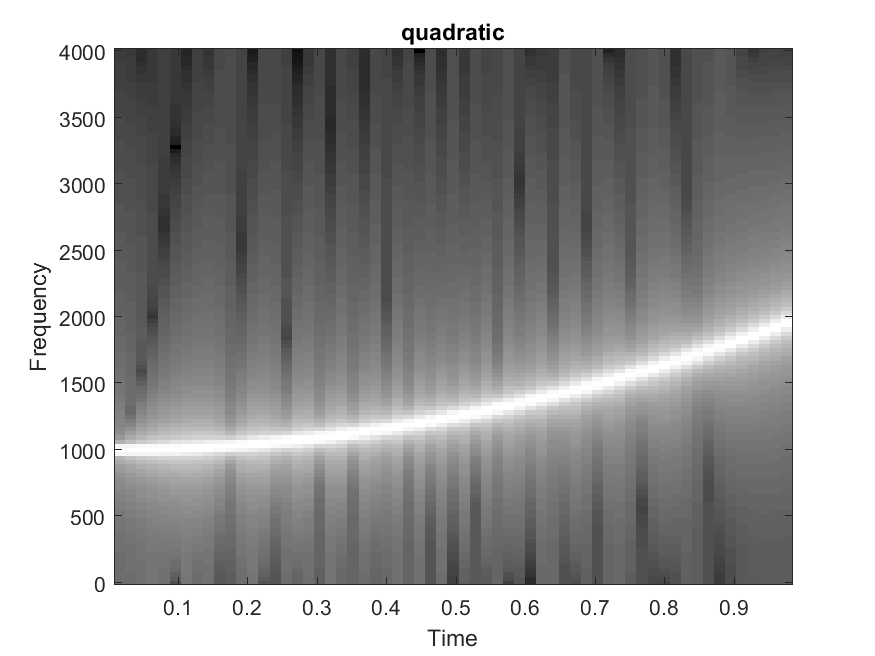
\includegraphics[scale=0.7]{graph11_2}
		\caption{Спектрограмма квадратичной функции chirp} 
		\label{pic:graph11_2} % название для ссылок внутри кода
	\end{center}
\end{figure}
\begin{figure}[H]
	\begin{center}
		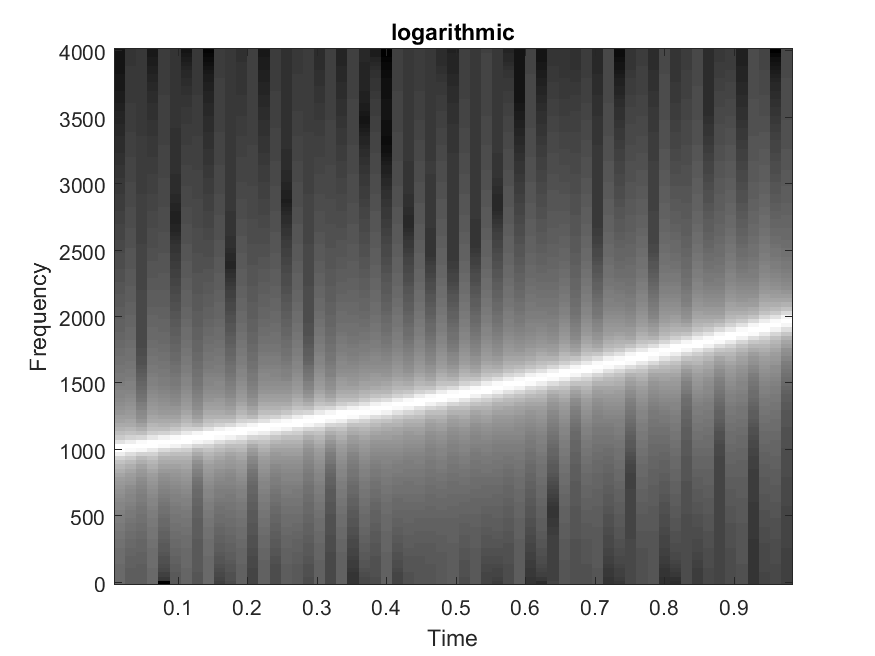
\includegraphics[scale=0.7]{graph11_3}
		\caption{Спектрограмма логарифмической функции chirp} 
		\label{pic:graph11_3} % название для ссылок внутри кода
	\end{center}
\end{figure}
На приведенных спектрограммах видно, что характер изменения мгновенной частоты сигнала совпадает с выбранной функцией.

\subsection{Сравнение методов корреляции}
Код использованный при сравнении алгоритмов находится в листинге~\ref{code:moduleCorr}.
В качестве исходного примера была взята задача нахождения синхропосылки 101 в сигнале 0001010111000010.
Перед началом вычисления корреляции синхропосылка была изменена - 1 0 1 на 1 -1 1 для ее более надежного нахождения в посылке, и дополнена нулями для совпадения длин двух векторов.
Далее производились 2 расчета корреляции - обычным алгоритмом и быстрым с контролем времени на каждую операцию.
Оба алгоритма показали, что синхропосылка была найдена в сигнале 2 раза - по смещению +3 и +5. 
Первый алгоритм показал время выполнения - 0,035 мс, в то время как второй - 0,017 мс. Можно сделать вывод, что
алгоритм быстрой корреляции эффективней обычного. Разница не значительна из-за малой длины посылки.

\section{Выводы}

В данной работе исследованы методы получения и визуализации различных сигналов в среде Matlab. 

Рассмотрены различные виды сигналов - детерминированные, периодические, конечные (финитные) и бесконечные, гармонические колебания и сигналы, полученные на их основе, единичные импульсы различной формы.

Получены спектры сигналов с помощью преобразования Фурье. Преобразование Фурье - одна из фундаментальных операций в телекоммуникационных технологиях, т.к. с его помощью можно быстро получать спектры сигналов для их анализа и модификации. 

Были опробованы 2 метода подсчета корреляции на простом примере. Стоит отметить,  на таком коротком примере алгоритм быстрой корреляции оказался всего в 2 раза быстрее обычного алгоритма. Его эффективность вырастет во много раз, по сравнению с 
обычным алгоритмом на больших посылках.
\newpage
\section{Листинг}

\lstinputlisting[
	label=code:module1,
	caption={Затухающий гармонический сигнал},
]{module1.m}
\parindent=1cm

\lstinputlisting[
	label=code:module2,
	caption={Сигналы, различающиеся по частоте },
]{module2.m}
\parindent=1cm

\lstinputlisting[
	label=code:module3,
	caption={Кусочные сигналы},
]{module3.m}
\parindent=1cm

\lstinputlisting[
	label=code:module5,
	caption={Прямоугольный сигнал},
]{module5.m}
\parindent=1cm

\lstinputlisting[
	label=code:module6,
	caption={Трапециевидный сигнал},
]{module6.m}
\parindent=1cm

\lstinputlisting[
	label=code:module7,
	caption={Импульс с ограниченной полосой частот},
]{module7.m}
\parindent=1cm

\lstinputlisting[
	label=code:module8,
	caption={Гауссов радиоимпульс},
]{module8.m}
\parindent=1cm

\lstinputlisting[
	label=code:module9,
	caption={Треугольные импульсы},
]{module9.m}
\parindent=1cm

\lstinputlisting[
	label=code:module10,
	caption={Гармонические импульсы},
]{module10.m}
\parindent=1cm

\lstinputlisting[
	label=code:module11,
	caption={Код для генерации периодического прямоугольного сигнала},
]{module11.m}
\parindent=1cm

\lstinputlisting[
	label=code:module12,
	caption={Код для генерации треугольных импульсов},
]{module12.m}
\parindent=1cm

\lstinputlisting[
	label=code:module13,
	caption={Функция Дирихле},
]{module13.m}
\parindent=1cm


\lstinputlisting[
	label=code:module14,
	caption={Код генерации сигнала с меняющейся частотой},
]{module14.m}
\parindent=1cm

\lstinputlisting[
	label=code:moduleCorr,
	caption={Код сравнения алгоритмов определения корреляции},
]{moduleCorr.m}
\parindent=1cm

\end{document}

